\documentclass{prova}

\usepackage{amsmath}
\usepackage{amsfonts}
\usepackage{tikz}

\setlength{\textheight}{25cm}

\renewcommand{\sin}{\,\mbox{sen}\,}
\newcommand{\ds}{\displaystyle}

\professor{Prof.\@ Adriano Barbosa}
\disciplina{C\'alculo de V\'arias Vari\'aveis}
\avaliacao{P2}
\curso{Matem\'atica}
\data{21/02/2024}

\begin{document}
	\cabecalho{5}  % o numero 5 indica a qnt de quadros na tabela de nota

    \textbf{Todas as respostas devem ser justificadas.}

    \begin{questionario}
        \q{(2 pts) Calcule a integral $\ds\iint_R x\sin(x+y)\ dA$, onde $R$ \'e a regi\~ao
           da figura abaixo.}
           \begin{figure}[h]
               \centering
               \scalebox{1.5}{
                   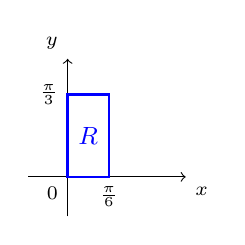
\begin{tikzpicture}
                       \draw[->] (-0.5,0) -- (1.5,0) node[anchor=north west] {\scriptsize$x$};
                       \draw[->] (0,-0.5) -- (0,1.5) node[anchor=south east] {\scriptsize$y$};
                       \draw (0,0) node[anchor=north east] {\scriptsize$0$};
                       \draw (pi/6,0) node[anchor=north] {\scriptsize$\frac{\pi}{6}$};
                       \draw (0,pi/3) node[anchor=east] {\scriptsize$\frac{\pi}{3}$};
                       \draw[thick,blue] (0,0) rectangle (pi/6,pi/3);
                       \draw[blue] (pi/6/2,pi/3/2) node {\small$R$};
                   \end{tikzpicture}
               }
           \end{figure}
        \q{(2 pts) Calcule a integral dupla $\ds\int_0^2\int_{-y}^{2y} xe^{y^3}\ dx dy$.}
        \q{(2 pts) Use coordenadas polares para determinar o volume do s\'olido acima do
           cone $z=-\sqrt{x^2+y^2}$ e abaixo do disco $x^2+y^2\le 4$.}
        \q{(2 pts) Calcule $\ds\iiint_E y\ dV$, onde $E$ \'e a regi\~ao do espa\c{c}o limitada
           pelos planos $x=0$, $y=0$, $z=0$ e $x+y+z=1$.}
        \q{Seja $E$ a regi\~ao limitada acima pela esfera $\rho=a$ e abaixo pelo
           cone $\phi=\frac{\pi}{3}$. Expresse a integral $\ds\iiint_E x^2+y^2\
           dV$ em:}
           \begin{questionario}
               \qq{(2/3 pt) Coordenadas esf\'ericas.}
               \qq{(2/3 pt) Coordenadas cil\'{\i}ndricas.}
               \qq{(2/3 pt) Coordenadas cartesianas.}
           \end{questionario}
    \end{questionario}
\end{document}
